\documentclass[a4paper]{article}
\usepackage[utf8]{inputenc}
\usepackage{amsmath}
\usepackage{graphicx}
\usepackage{indentfirst}
\usepackage{subfig}
\usepackage{float} % para usar [H]
%opening

\begin{document}

\noindent UNIVERSIDAD SIMÓN BOLÍVAR\\
Departamento de Cómputo Científico\\
CO-6612, Introducción a las redes neuronales\\
Tarea 2: Clasificadores lineales\\
María Victoria Jorge\\
11-10495

\section{Clasificadores Lineales}
	En esta sección se presentarán los experimentos realizados para construir clasificadores lineales mediante aprendizaje con reforzamiento, un perceptrón de una capa y un adaline.\\
	
	Para medir la calidad de todos los modelos se utilizará la técnica de validación cruzada. Además, se utilizará el porcentaje de datos bien clasificados como métrica de \textit{performance}. Por último, para asegurarnos que los modelos no están aprendiendo a clasificar basándose en el orden en el que reciben los datos, en cada corrida estos se desordenarán aleatoriamente.\\
	
	Como los datos presentados en el archivo lincloud3 tienen solo dos dimensiones, pueden graficarse e identificar fácilmente si
	son linealmente separables, para asegurarnos que los modelos utilizados a continuación serán capaces de clasificarlos. En la figura \ref{fig:datosOriginales} se tienen todos los datos identificados según la clase a la que pertenecen, y se puede observar que es posible trazar una línea entre ambas clases para separarlas.
	
	\begin{figure}[H]
	  \centering
	  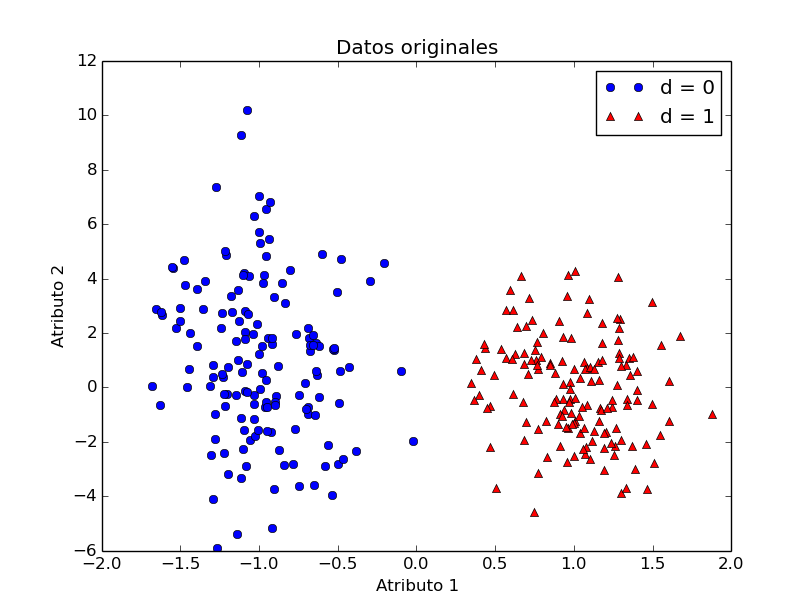
\includegraphics[scale=0.4]{datos.png}
	  \caption{Datos originales}
	  \label{fig:datosOriginales}
	\end{figure}
	
	\subsection{Aprendizaje con reforzamiento}
		Para estas pruebas se inicializaron los pesos de las dos neuronas en valores aleatorios entre -0.5 y 0.5, y se usaron esos mismos valores en todas las corridas. Como condición de parada para el entrenamiento se tomó que no existiera error en la clasificación de los datos o que se superara un número máximo de épocas (1000 épocas).\\
		
		En la Tabla \ref{tabla:accReforzamiento} están los resultados obtenidos de la ejecución de la validación cruzada 5-fold usando la red basada en aprendizaje con reforzamiento. Se observa que para las tres tasas de aprendizaje utilizadas se obtuvieron resultados parecidos, clasificando correctamente la mayoría de los datos. El número de épocas indicado es el promedio de épocas utilizadas durante las 5 iteraciones de la validación cruzada.
		\begin{table}[H]
		\begin{center}
		\begin{tabular}{|l|l|l|l|l|}
		\hline
		Total datos & $\alpha$ & \% Correctos & \% Incorrectos & Épocas\\
		\hline \hline
		300 & 0.1 & 99.6667 & 0.3333 & 4.8 \\ \hline
		300 & 0.01 & 99.6667 & 0.3333 & 2\\ \hline
		300 & 0.001 & 99.3333 & 0.6667 & 4.2\\ \hline
		\end{tabular}
		\caption{Exactitud aprendizaje con reforzamiento}
		\label{tabla:accReforzamiento}
		\end{center}
		\end{table}
	
	\subsection{Perceptrón}
		Para estas pruebas se inicializaron los pesos en valores aleatorios entre -0.5 y 0.5, y se usaron esos mismos valores en todas las corridas. Se utilizó una sola neurona y la función de activación sgn o umbral. Como condición de parada para el entrenamiento se tomó que no existiera error en la clasificación de los datos o que se superara un número máximo de épocas (1000 épocas). Además se cambió la respuesta deseada de los datos cuyo valor era 0, por -1, para mantener la simetría respecto al 0 y que ambas clases tuvieran el mismo peso.\\
		
		En la Tabla \ref{tabla:accPerceptron} se pueden observar los resultados obtenidos luego de ejecutar validación cruzada con 5-fold para diferentes tasas de aprendizaje en una única neurona. Por cada iteración se utilizaron 240 datos para entrenar y 60 para probar el modelo. Luego de 5 iteraciones se probó en todos los experimentos con los 300 datos. El número de épocas indicado para cada tasa de aprendizaje es el promedio de los 5 entrenamientos realizados por tasa, con diferentes datos para entrenar en cada una.\\
		
		\begin{table}[H]
		\begin{center}
		\begin{tabular}{|l|l|l|l|l|}
		\hline
		Total datos & $\alpha$ & \% Correctos & \% Incorrectos & Épocas\\
		\hline \hline
		300 & 0.1 & 99.6666 & 0.3334 & 3\\ \hline
		300 & 0.01 & 99.6666 & 0.3334 & 3.4\\ \hline
		300 & 0.001 & 99.3333 & 0.6667 & 15.2\\ \hline
		\end{tabular}
		\caption{Exactitud del perceptrón}
		\label{tabla:accPerceptron}
		\end{center}
		\end{table}
		
		Con estos resultados puede observarse que al disminuir la tasa de aprendizaje el perceptrón necesita más épocas para cumplir con la cota de clasificar correctamente todos los datos de entrenamiento. Sin embargo, parece que al aumentar la cantidad de épocas para estos datos, el perceptrón tiene más problemas para clasificar los datos nuevos.\\
					
		Esto puede apreciarse de forma más clara en las gráficas de la figura \ref{f:perceptron}, donde se muestra para cada tasa de aprendizaje utilizada el peor hiperplano generado de todas las iteraciones de la validación cruzada. Podemos observar que en las tres figuras el hiperplano está muy cerca de las dos fronteras, lo que puede originar errores de clasificación cuando esos datos no se encuentran dentro del conjunto de entrenamiento, como sucedió en las gráficas \ref{f:perceptron2} y \ref{f:perceptron3}. Con esto se puede concluir que el modelo tiene problemas para generalizar.			
				
		\begin{figure}[H]
		 \centering
		  \subfloat[$\alpha=0.1$]{
		   \label{f:perceptron1}
		    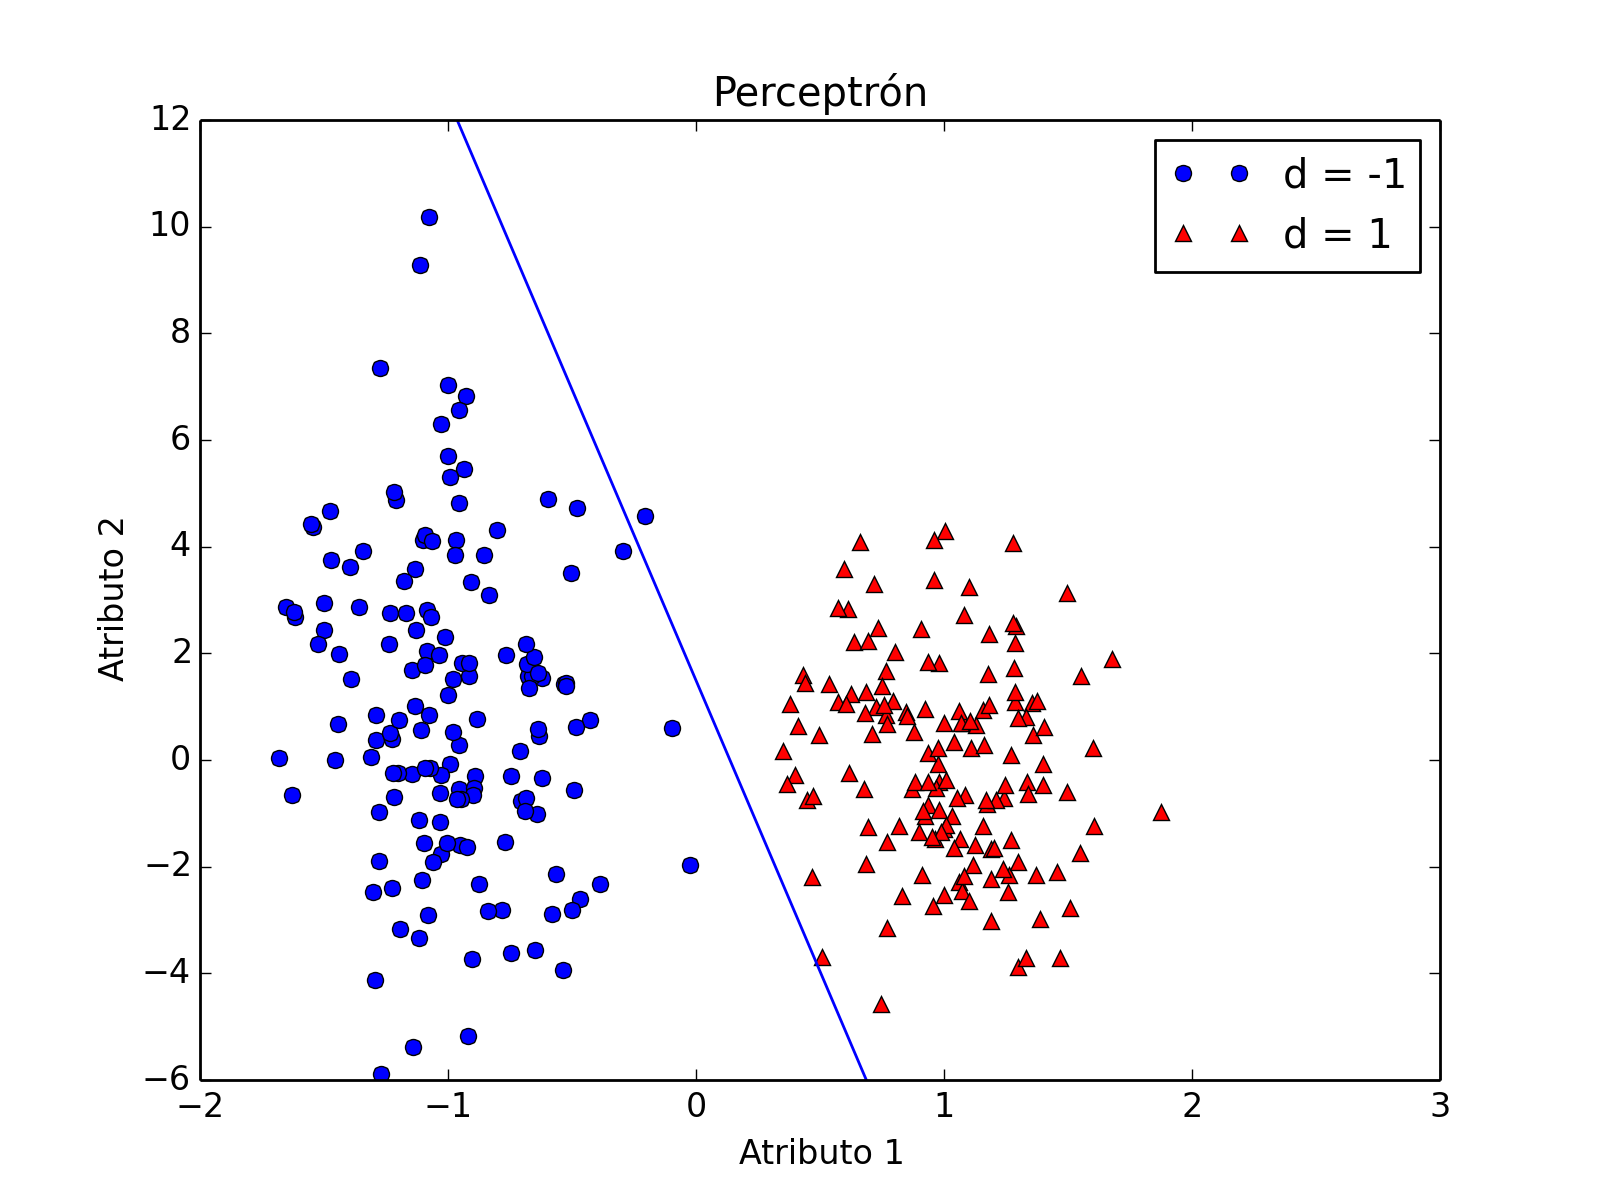
\includegraphics[width=0.3\textwidth]{perceptron.png}}
		  \subfloat[$\alpha=0.01$]{
		   \label{f:perceptron2}
		    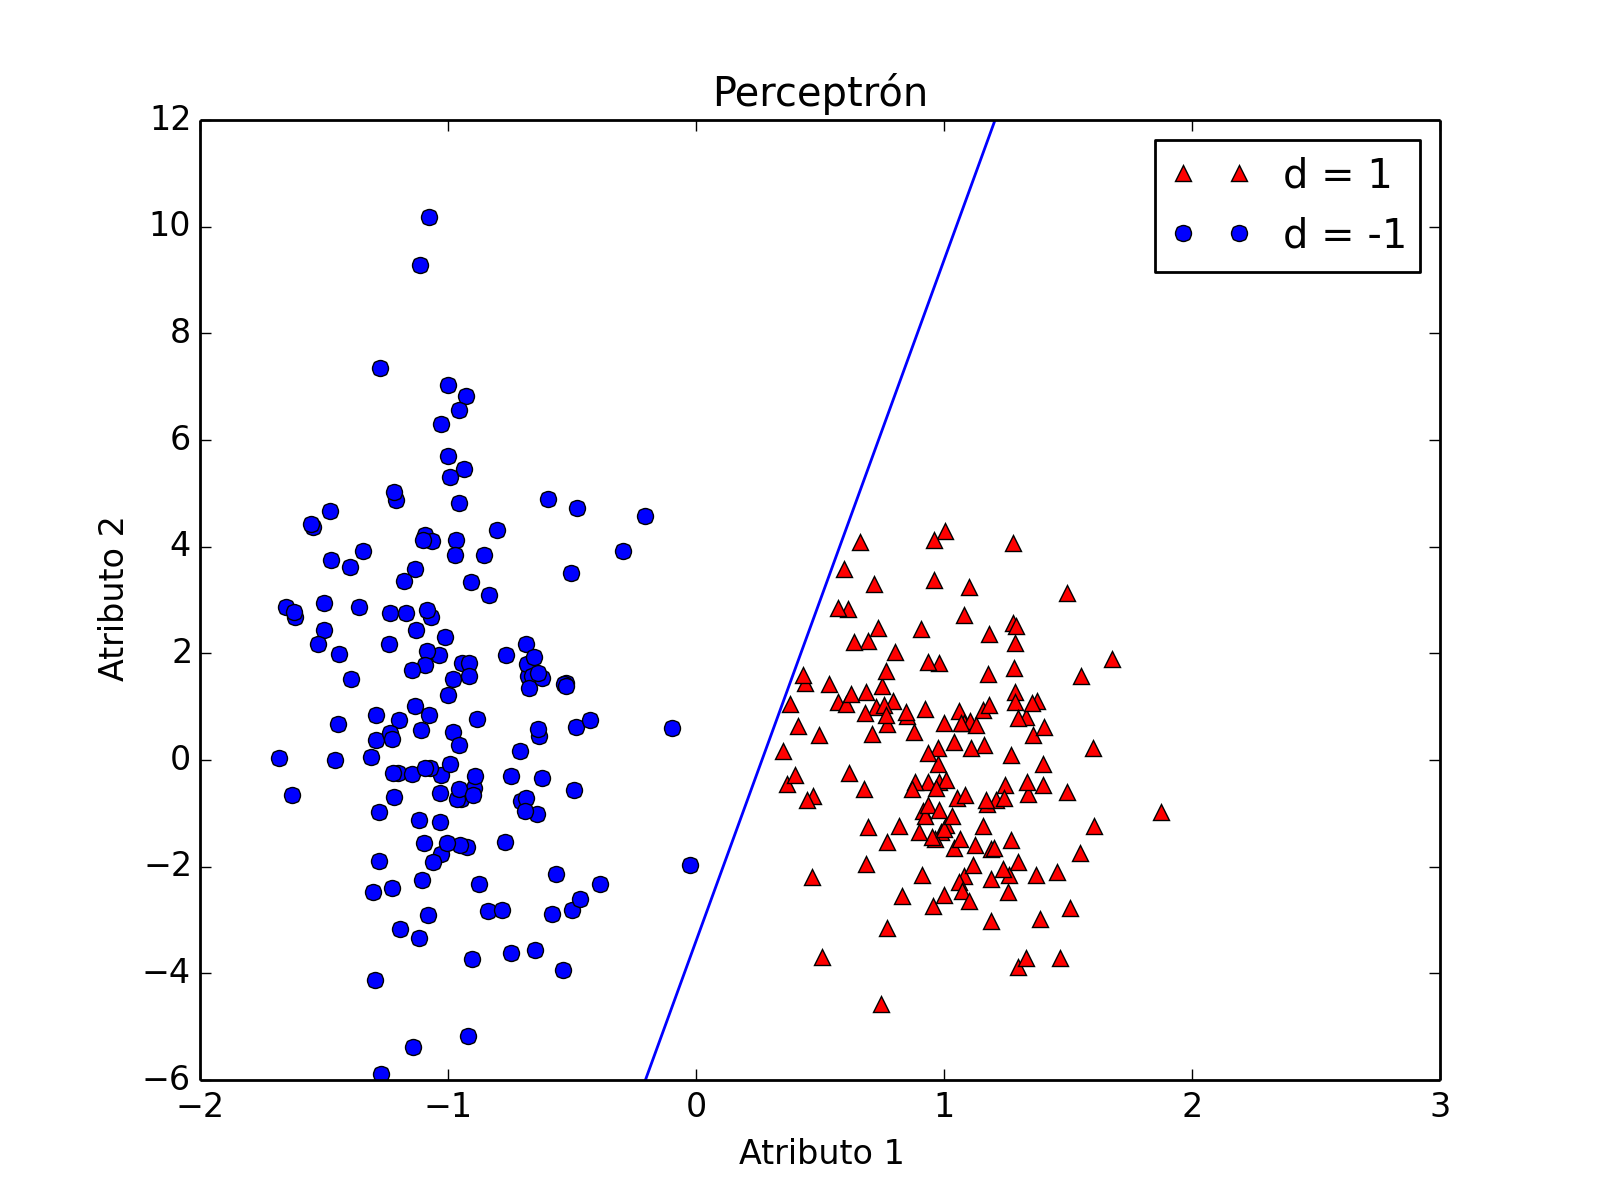
\includegraphics[width=0.3\textwidth]{perceptron_01.png}}
		  \subfloat[$\alpha=0.001$]{
		   \label{f:perceptron3}
		    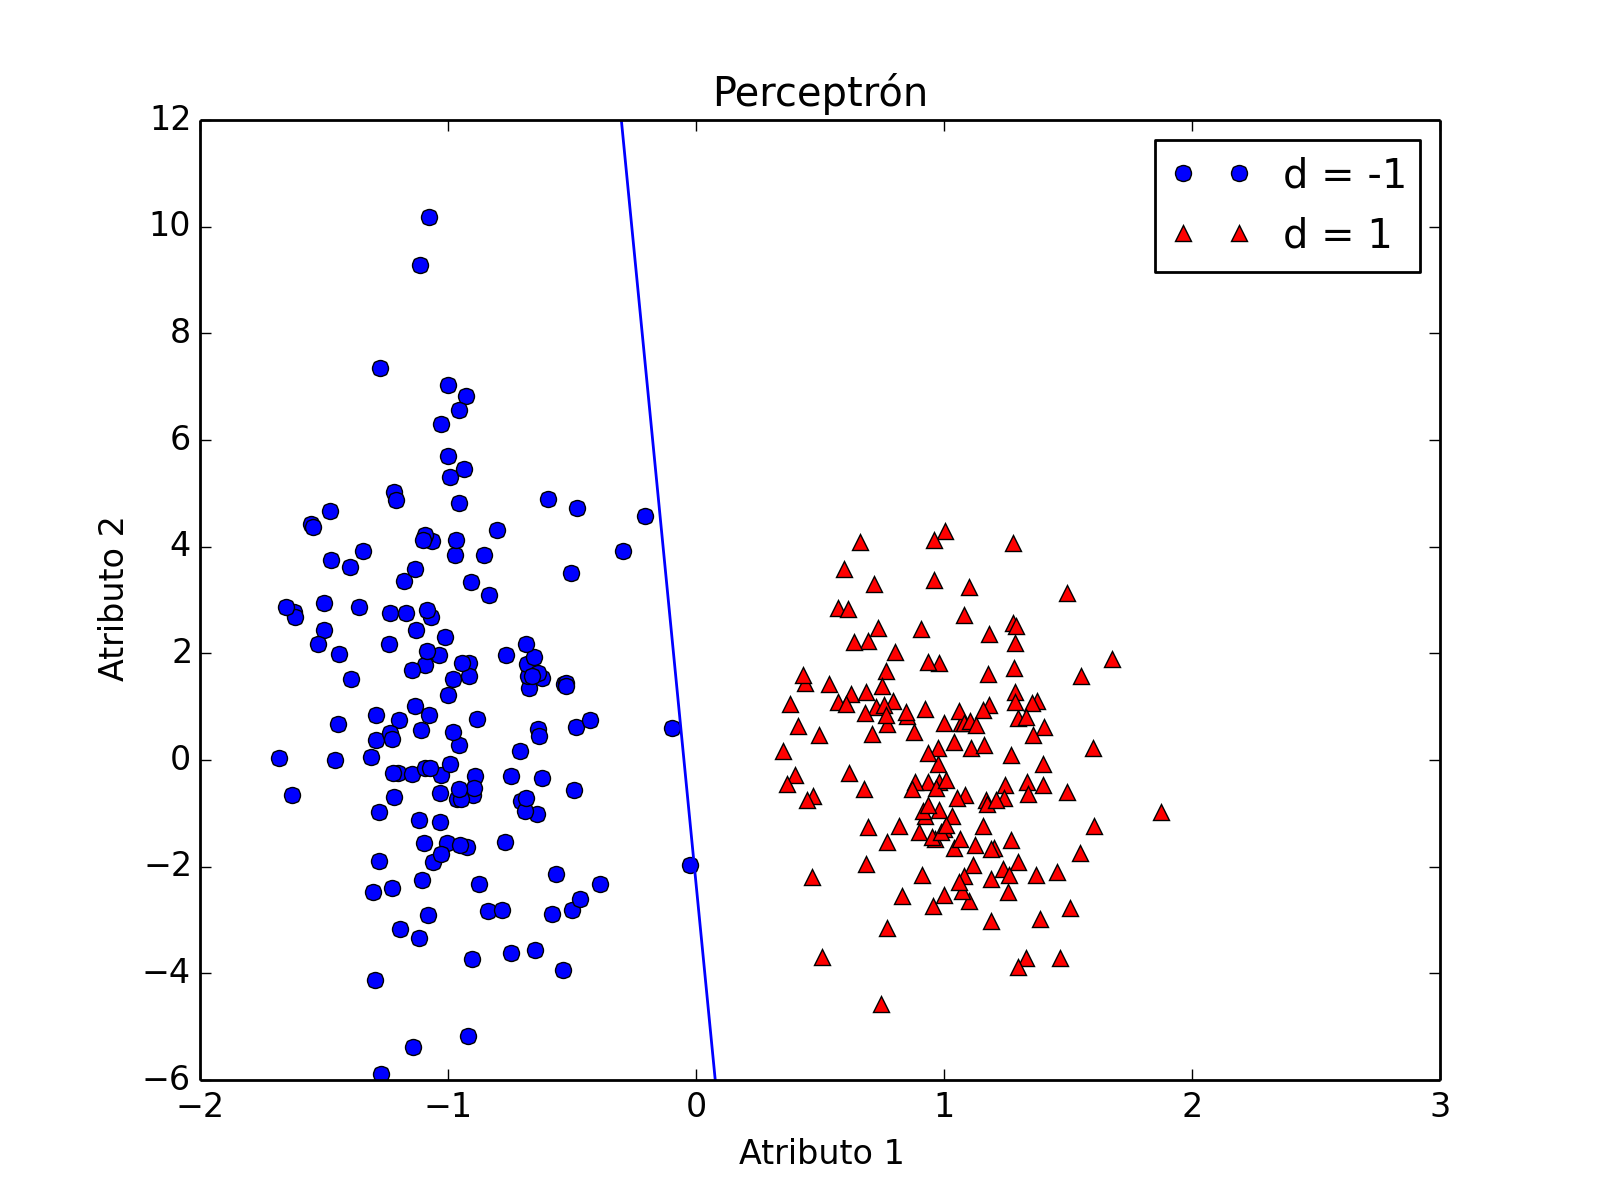
\includegraphics[width=0.3\textwidth]{perceptron_001.png}}
		 \caption{Modelos de perceptrón obtenidos en los tres experimentos}
		 \label{f:perceptron}
		\end{figure}
	
	\subsection{Adaline}
		Para estas pruebas se inicializaron los pesos de la neurona en valores aleatorios entre -0.5 y 0.5, manteniéndolos fijos durante todas las iteraciones de la validación cruzada de 5-fold. Como condición de parada para el algoritmo de entrenamiento se usó un máximo de 5000 épocas. Además, se modificó el archivo que contiene los datos para que las clases sean -1 y 1, en vez de 0 y 1 como estaban originalmente.\\
		
		En la Tabla \ref{tabla:accAdaline} se encuentran los resultados obtenidos para diferentes tasas de aprendizaje.
		Se puede observar que con tasas de aprendizaje muy pequeñas el Adaline converge mejor a la solución esperada, clasificando correctamente todos los datos.
		\begin{table}[H]
		\begin{center}
		\begin{tabular}{|l|l|l|l|l|}
		\hline
		Total datos & $\alpha$ & \% Correctos & \% Incorrectos & Épocas\\
		\hline \hline
		300 & 0.1 & 98 & 2 & 5000\\ \hline
		300 & 0.01 & 100 & 0 & 5000\\ \hline
		300 & 0.001 & 100 & 0 & 5000\\ \hline
		\end{tabular}
		\caption{Exactitud del Adaline}
		\label{tabla:accAdaline}
		\end{center}
		\end{table}
		
		Se realizaron pruebas con otras tasas de aprendizaje pero se presentaron solo las más significativas. El valor más alto con el que se obtuvieron buenos resultados fue $\alpha=0.1$. Con $\alpha$ más grandes, 5000 épocas no son suficientes para que el Adaline genere porcentajes tan altos de aciertos, debido a que se le dificulta la convergencia.\\
		
		Al igual que para el Perceptrón, se graficaron los hiperplanos generados en los experimentos para el Adaline. En la figura \ref{f:adaline} se encuentran los peores de cada validación cruzada para cada una de las tasas de aprendizaje utilizadas. Puede observarse en la figura \ref{f:adaline1} que ya la tasa de aprendizaje 0.1 puede ser muy alta dependiendo de la diversidad del conjunto de entrenamiento. En ese caso los valores más cercanos a la frontera no se encontraban en dicho conjunto lo que ocasionó una mala generalización del modelo.
		
		\begin{figure}[H]
		\centering
		\subfloat[$\alpha=0.1$]{
		\label{f:adaline1}
		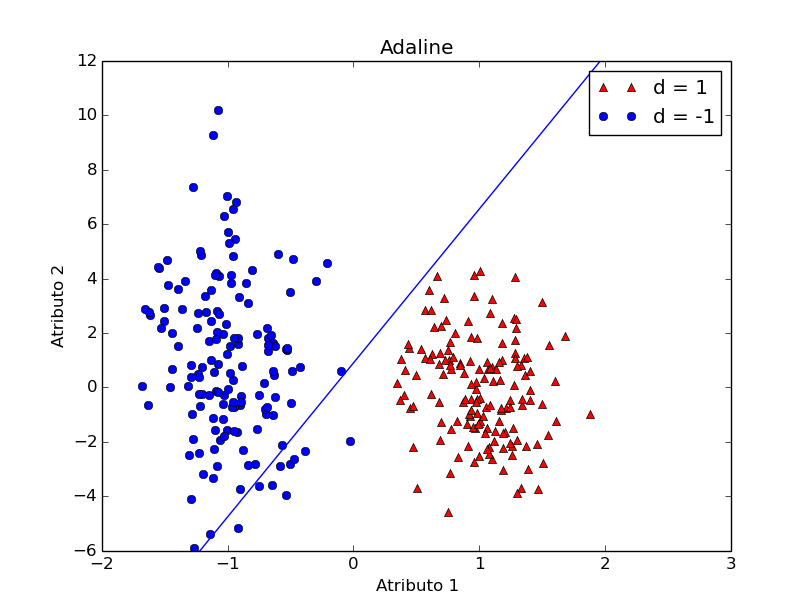
\includegraphics[width=0.3\textwidth]{adaline_1.png}}
		\subfloat[$\alpha=0.01$]{
		\label{f:adaline01}
		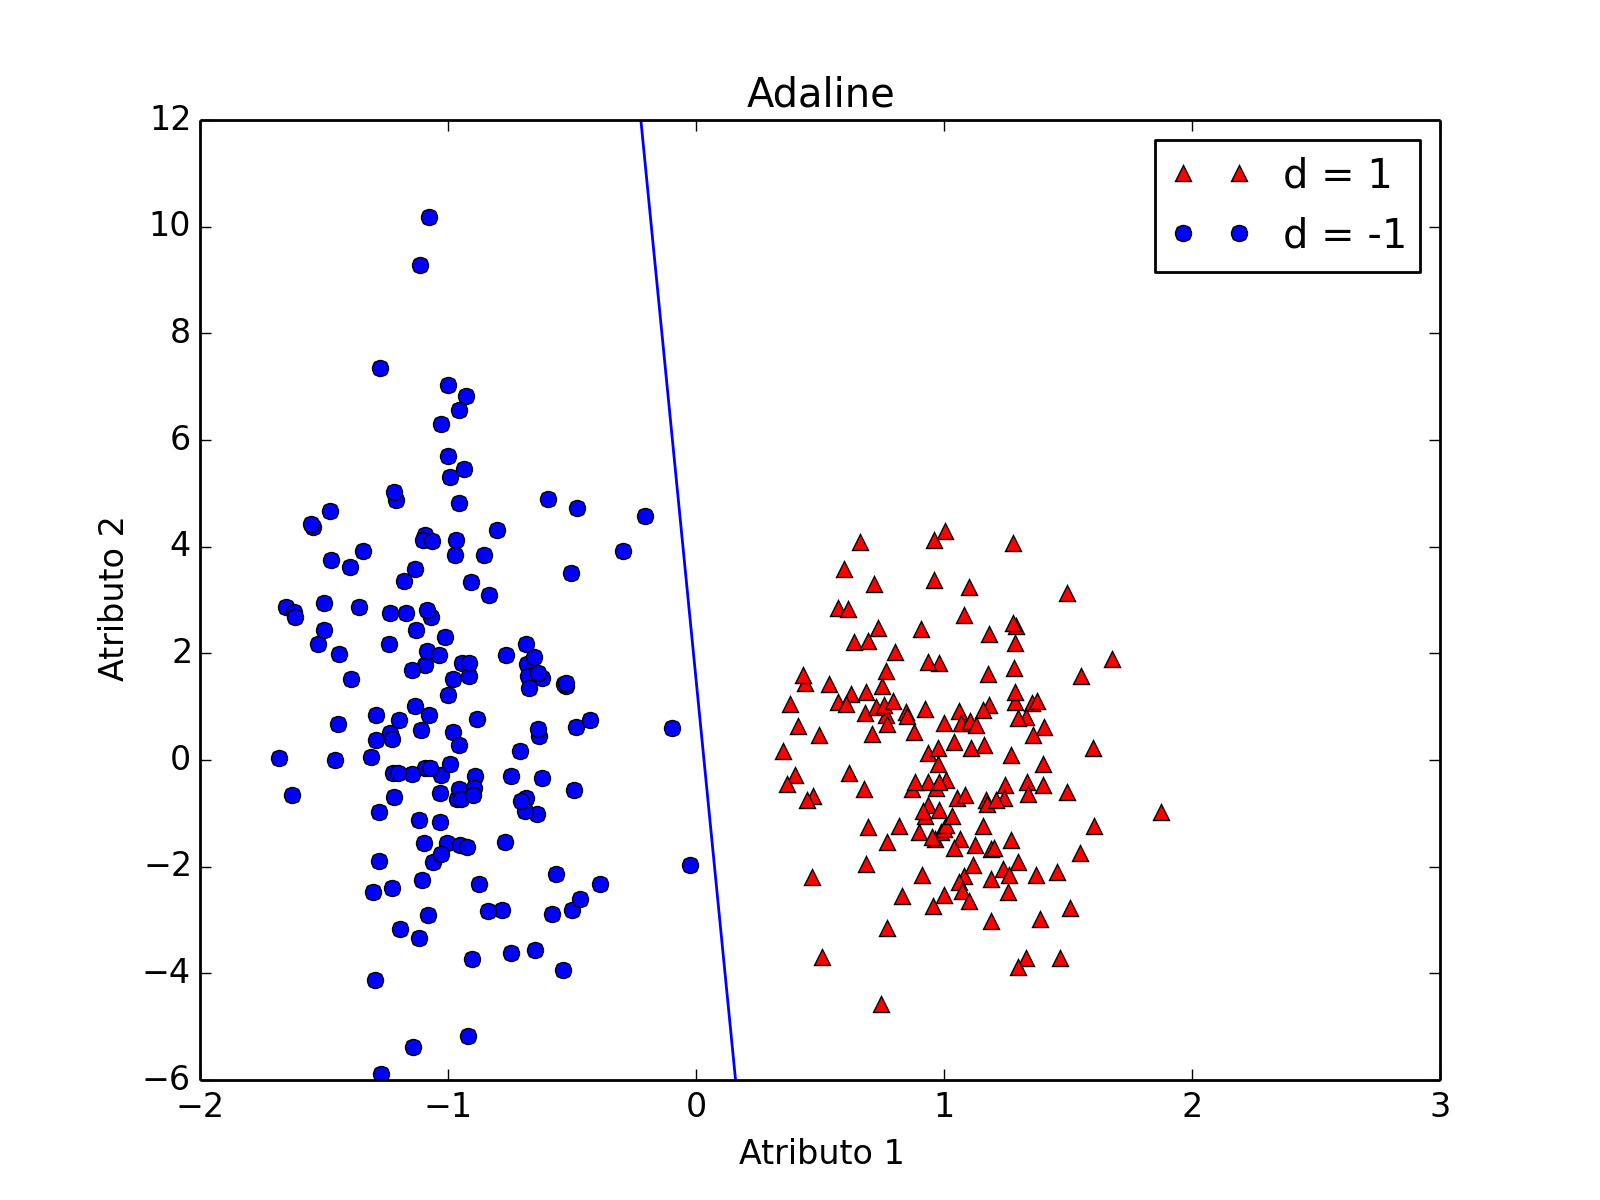
\includegraphics[width=0.3\textwidth]{adaline_01.png}}
		\subfloat[$\alpha=0.001$]{
		\label{f:adaline001}
		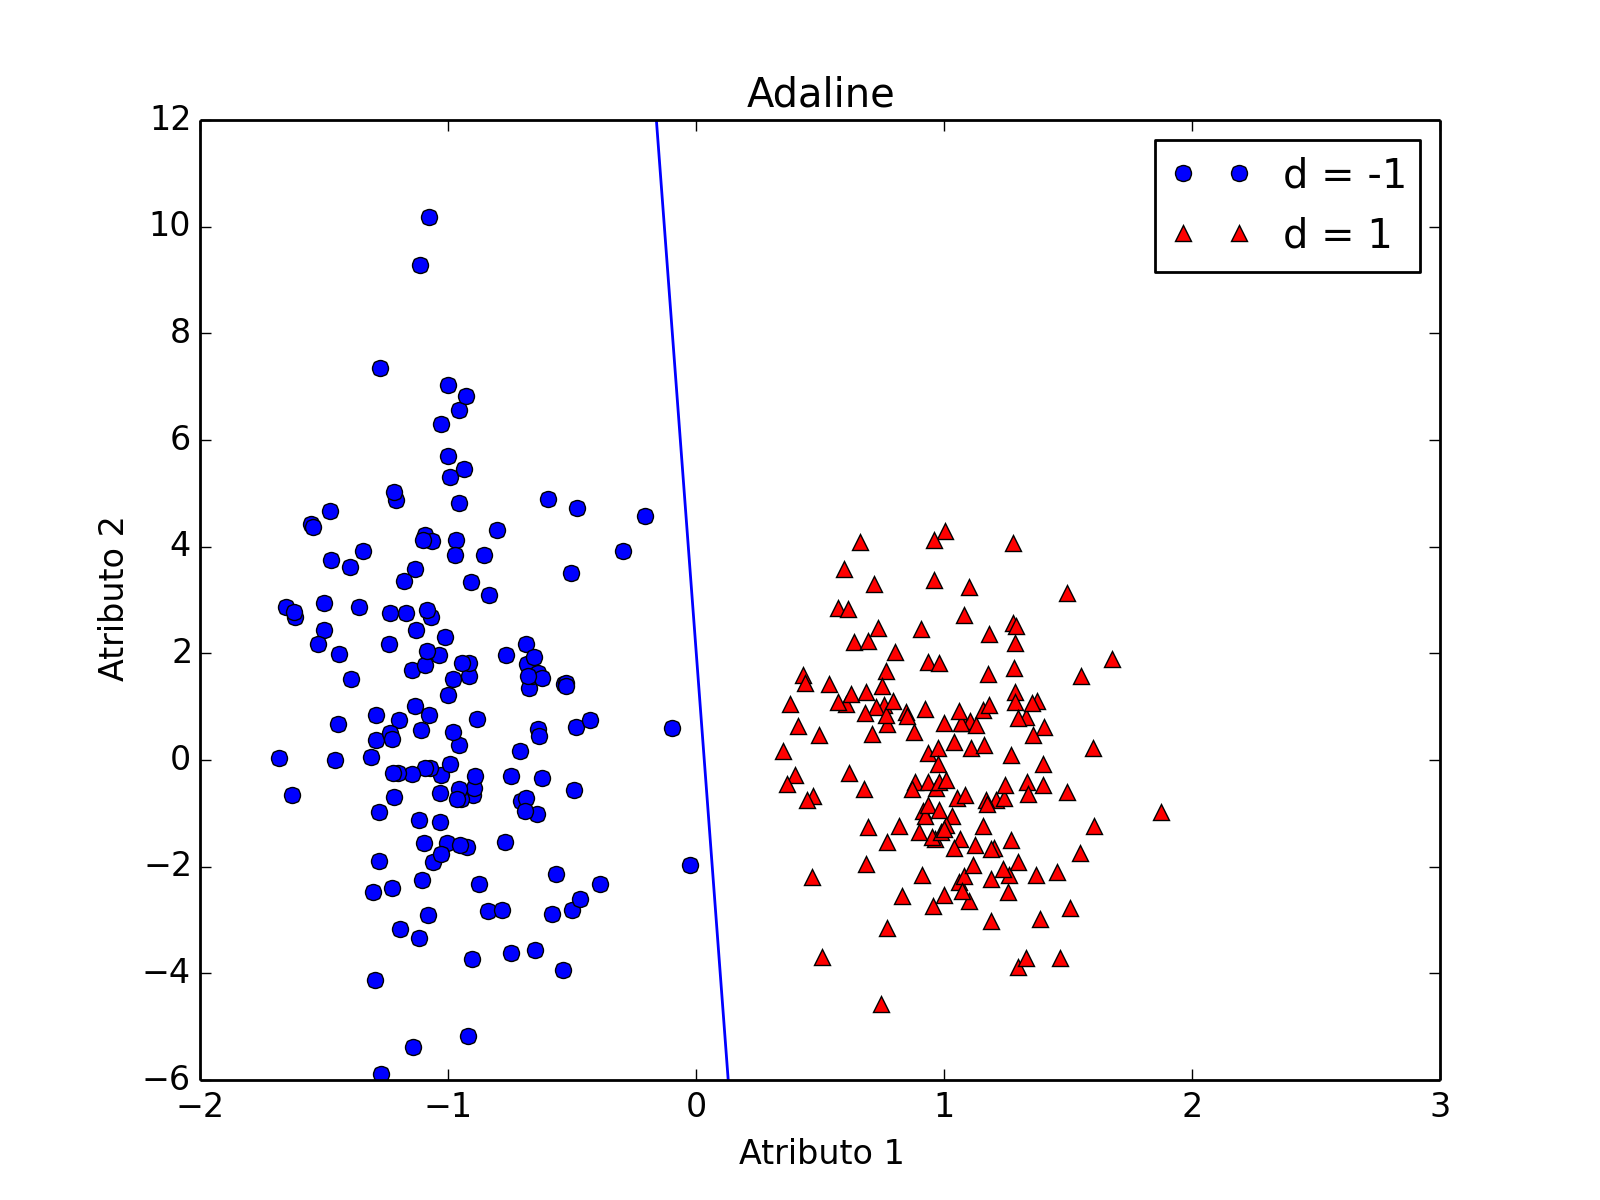
\includegraphics[width=0.3\textwidth]{adaline_001.png}}
		\caption{Modelos de Adaline obtenidos en los tres experimentos}
		\label{f:adaline}
		\end{figure}
	
\section{Interpolador}
	El algoritmo de Adaline puede ser utilizado para iterpolación de funciones si se calcula la salida de la siguiente forma $y = a + b_{1}x + b_{2}x^{2} + ... + b_{k}x^{k}$, siendo k el grado del polinomio que se usará para interpolar, 'a'  el sesgo, y cada $b_{i}$ los $w_{i}$ del Adaline.\\
	
	Sabiendo esto debemos conocer cómo se comportan los datos que tenemos en p3data para saber el grado del polinomio con el que aproximaremos la función que los originó. Con la figura \ref{fig:interpolador} se puede apreciar que los datos parecen ser originados por una función de grado impar, aún cuando tengan algo de ruido. Es por esto que se realizarán pruebas con polinomios de grado 3 y 5 con diferentes tasas de aprendizaje para determinar cuál verdaderamente aproxima mejor estos datos.
	
	\begin{figure}[H]
	\centering
	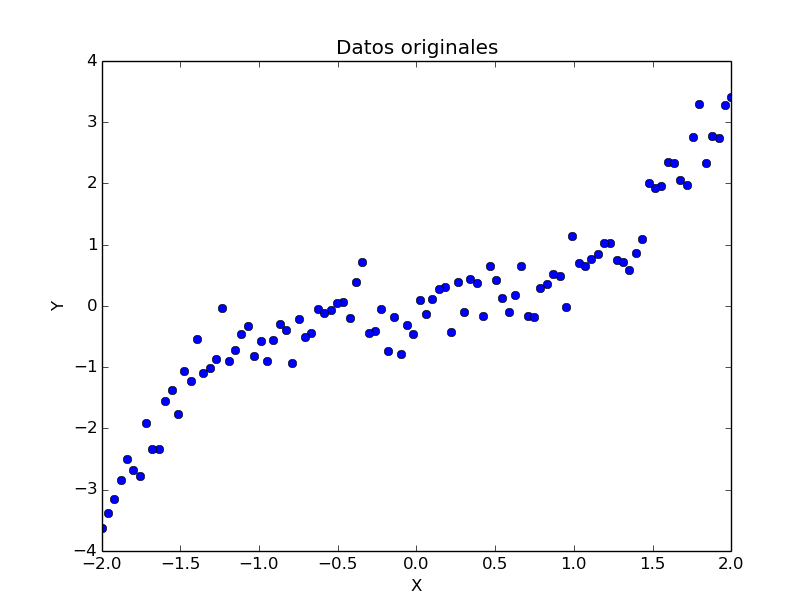
\includegraphics[scale=0.3]{interpolado.png}
	\caption{Datos originales a interpolar}
	\label{fig:interpolador}
	\end{figure}
	
	Usando una tasa de aprendizaje de 0.01 se obtuvieron los resultados presentes en la figura \ref{f:interpolado01}. Allí podemos observar las aproximaciones realizadas con los polinomios de grado 3 en \ref{f:tres01} y de grado 5 en \ref{f:cinco01}.
	
	\begin{figure}[H]
	\centering
	\subfloat[Polinomio grado 3]{
	\label{f:tres01}
	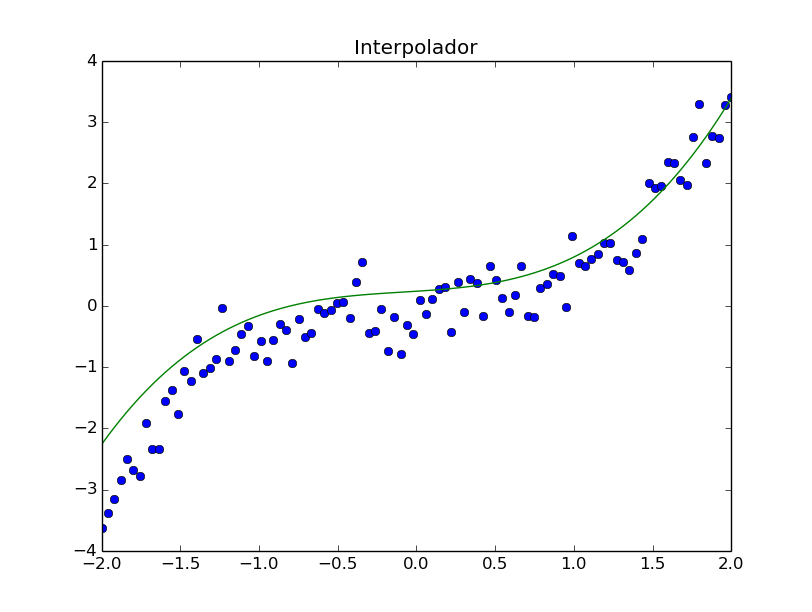
\includegraphics[width=0.5\textwidth]{interpolado3_01.png}}
	\subfloat[Polinomio grado 5]{
	\label{f:cinco01}
	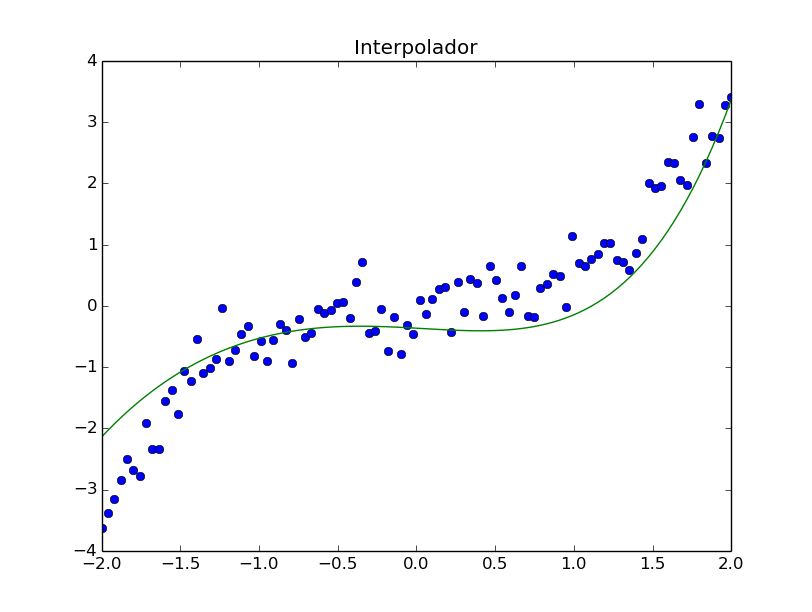
\includegraphics[width=0.5\textwidth]{interpolado5_01.png}}
	\caption{Interpoladores con $\alpha = 0.01$}
	\label{f:interpolado01}
	\end{figure}	
	
	Los resultados producto de los mismos polinomios pero con una tasa de aprendizaje para el Adaline de 0.001 se presentan en la figura \ref{f:tres001}.
	
	\begin{figure}[H]
	\centering
	\subfloat[Polinomio grado 3]{
	\label{f:tres001}
	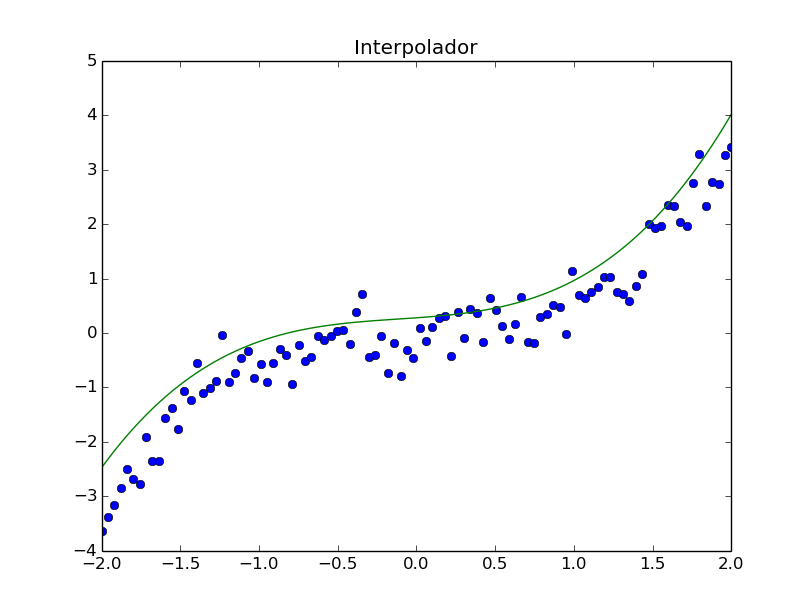
\includegraphics[width=0.5\textwidth]{interpolado3_001.png}}
	\subfloat[Polinomio grado 5]{
	\label{f:cinco001}
	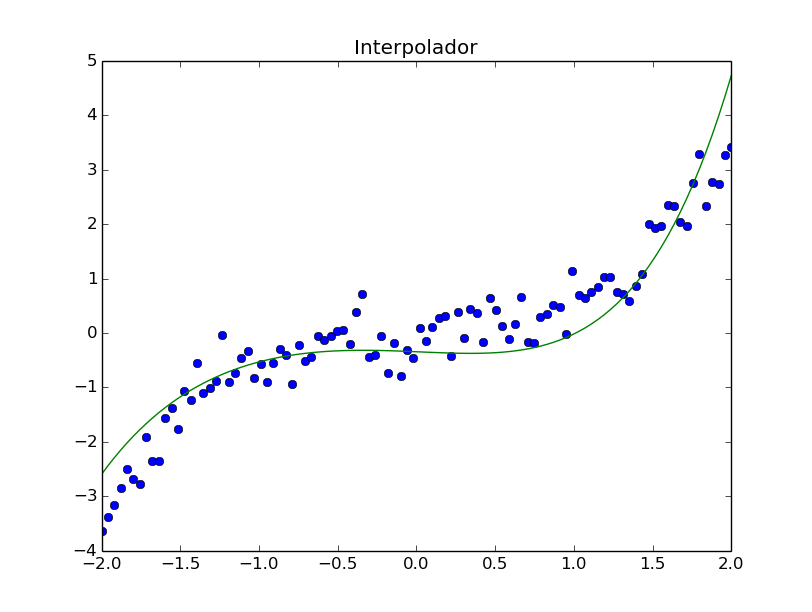
\includegraphics[width=0.5\textwidth]{interpolado5_001.png}}
	\caption{Interpoladores con $\alpha = 0.001$}
	\label{f:interpolado001}
	\end{figure}	
	
	El polinomio de grado 3 parece ser el que mejor moldea la forma de los datos, sin embargo parece estar desplazado hacia arriba por la presencia de datos que contienen ruido. Por otro lado, aunque el polinomio de grado 5 tiene curvas más pronunciadas, parece estar más cerca del centro de los datos, teniendo su mejor aproximación con $\alpha = 0.001$.
	
	

\section{O-exclusivo}
Se demostrará que las clases del O-exclusivo (XOR) no son linealmente separables por reducción al absurdo.\\

Supongamos entonces que las clases del XOR son linealmente separables. Entonces existe un $\vec{w} = [w_{0}, w_{1}, w_{2}]^{t}$ que permite generar el hiperplano $\vec{w}^{t}\vec{x} = 0$ para un perceptrón de una neurona. Esta es la frontera que divide a las dos clases del XOR. Los datos que estén por debajo de esa frontera pertenecen a la clase 0, y los que están por encima pertenecen a la clase 1.\\

Por lo tanto se generan las siguientes ecuaciones:\\
\begin{equation}
0*w_{1} + 0*w_{2} + w_{0} <= 0 \iff w_{0} <= 0
\end{equation}
\begin{equation}
0*w_{1} + 1*w_{2} + w_{0} > 0 \iff w_{0} > -w_{2}
\end{equation}
\begin{equation}
1*w_{1} + 0*w_{2} + w_{0} > 0 \iff w_{0} > -w_{1}
\end{equation}
\begin{equation}
1*w_{1} + 1*w_{2} + w_{0} <= 0 \iff w_{0} <= -w_{1} - w_{2}
\end{equation}\\

De (1) obtenemos que $w_{0}$ es un número no positivo. Usando esta información en (2) y (3) tenemos que $w_{1}$ y $w_{2}$ son números positivos. \\

Luego, sabiendo que $w_{1}$ es positivo, podemos asegurar que $-w_{2} > -w_{2} -w_{1}$. Usando esta cota inferior en (2) se sigue cumpliendo que $w_{0} > -w_{2} - w_{1}$. Esto entra en contradicción con (4) que se obtuvo directamente del perceptrón. Por lo tanto la suposición que se hizo inicialmente sobre la separabilidad lineal de las clases del XOR es errónea.

\section{Descenso del gradiente}
Considerando la función de costo $$E(w) = \frac{1}{2}\sigma^{2} - r^{t}w + \frac{1}{2}w^{t}Rw$$ sabemos que el vector de pesos tiene dos componentes $w_{1}$ y $w_{2}$. Si desarrollamos la función de costo para dejarlo en función de estas componentes nos queda:
$$E(w) = \frac{1}{2}\sigma{2} - \left[\begin{array}{cc}
0.8182 & 0.354\end{array}\right]\left[\begin{array}{c}
w_{1}
\\
w_{2}
\end{array}\right] + \frac{1}{2}\left[\begin{array}{cc}
w_{1} & w_{2}\end{array}\right]\left[\begin{array}{cc}
1 & 0.8182\\
0.8182 & 1
\end{array}\right] \left[\begin{array}{c}
w_{1}
\\
w_{2}
\end{array}\right]$$
$$= \frac{1}{2}\sigma^{2} - (0.8182w_{1}+0.354w_{2}) + \frac{1}{2}\left[\begin{array}{cc}
w_{1} + 0.3182w_{2} & 0.8182w_{1} + w_{2}
\end{array}\right]\left[\begin{array}{c}
w_{1}
\\
w_{2}
\end{array}\right]$$
$$= \frac{1}{2}\sigma^{2} - 0.8182w_{1} -0.354w_{2} + \frac{1}{2}(w_{1}^{2} + 1.6364w_{1}w_{2} + w_{2}^{2})$$

Luego, para encontrar el valor óptimo de w para el cual E(w) es mínimo debemos calcular el gradiente de la función de costo e igualarlo a cero para determinar los valores que deben tener $w_{1}$ y $w_{2}$.

\begin{equation}
\frac{\partial E(w)}{\partial w_{1}} = -0.8182 + w_{1} + \frac{16364}{2}w_{2} = 0
\end{equation} 
\begin{equation}
\frac{\partial E(w)}{\partial w_{2}} = -0.354 + w_{2} + \frac{1.6364}{2}w_{1} = 0
\end{equation}

Despejando $w_{1}$ de (5) obtenemos,
\begin{equation}
w_{1} = 0.8182(1 - w_{2})
\end{equation}

Luego, sustituyendo en (6):

$$-0.354 + w_{2} + 0.8182*0.8182(1-w_{2}) = 0$$

De donde obtenemos que $w_{2} = -0.9543$ y sustituyendo en (7) obtenemos que $w_{1} = 1.599$.\\

Ahora calcularemos el valor óptimo a través del algoritmo del Descenso del Gradiente. Para ambos experimentos se utilizó una precisión de 0.0001.
\begin{itemize}
\item $\eta = 0.3$\\
En la figura \ref{fig:gradient2_w1} se encuentra la trayectoria de la evolución de los valores de $w_{1}$ durante la ejecución del algoritmo. Los puntos indican los valores que tomó esta componente durante todas las iteraciones y la línea indica la trayectoria realizada.

	\begin{figure}[H]
	\centering
	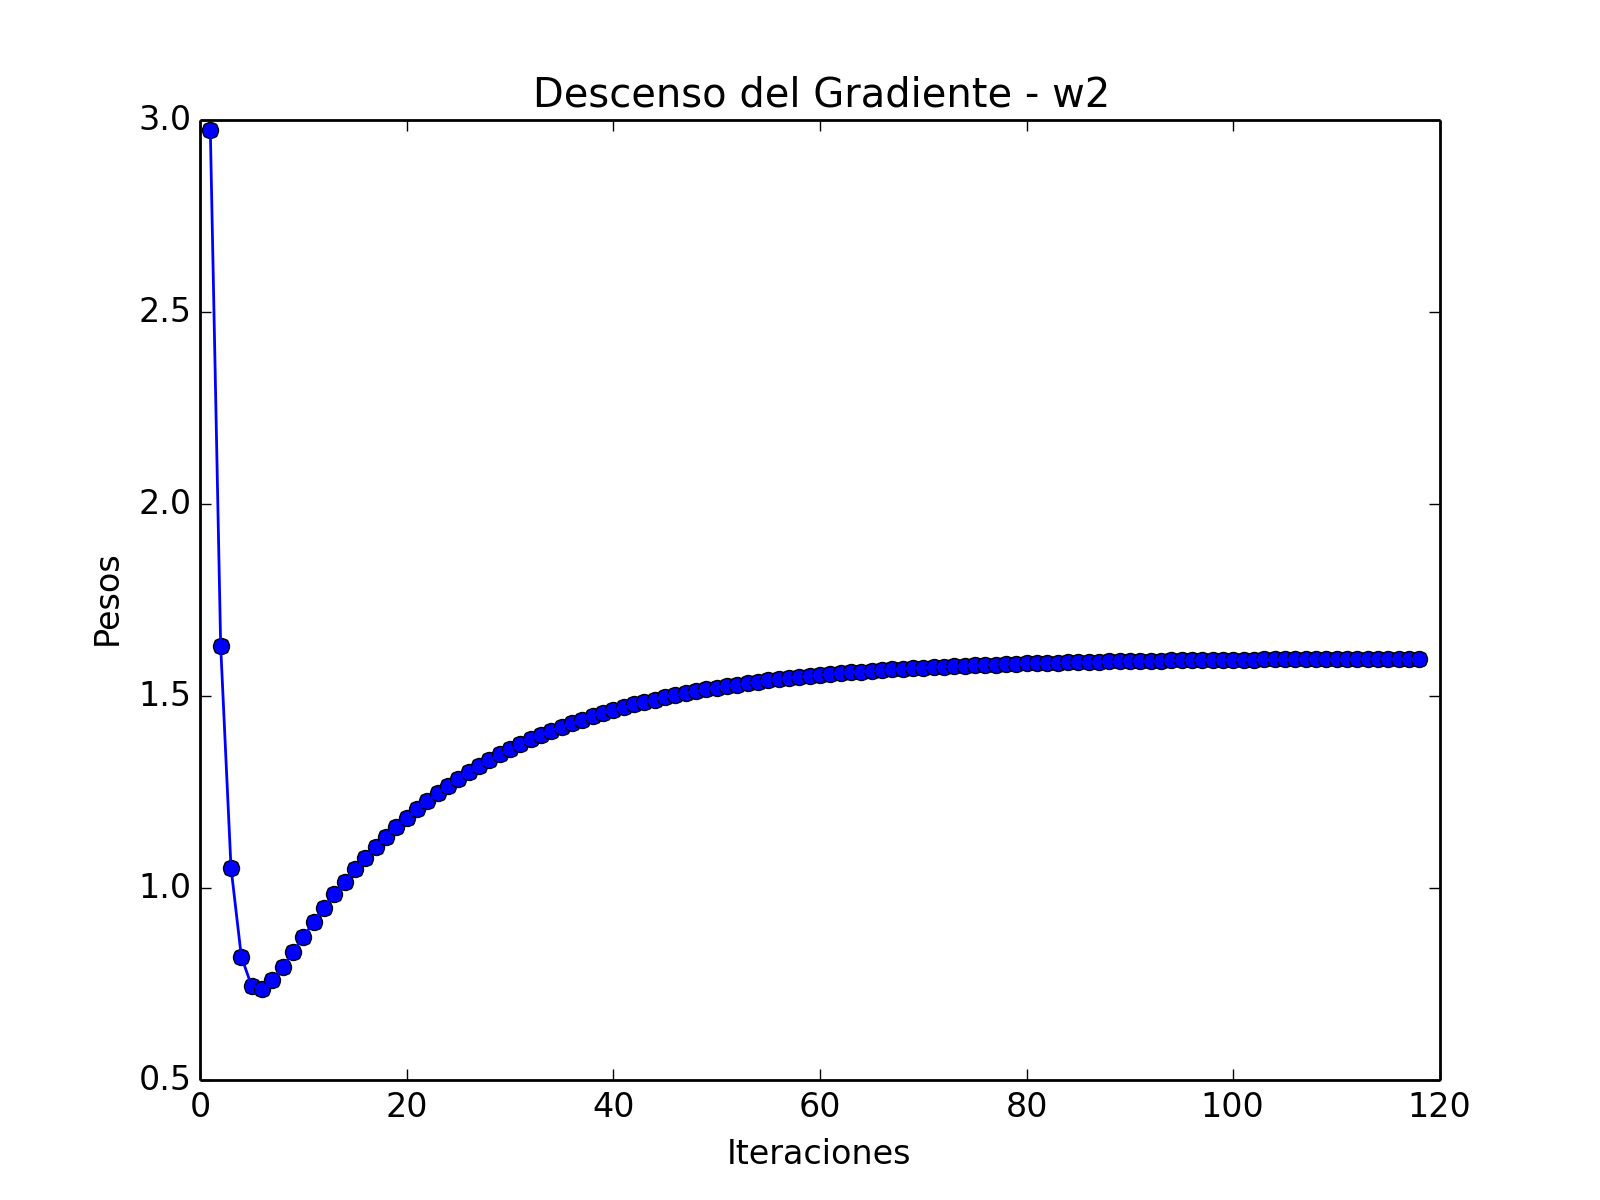
\includegraphics[scale=0.5]{gd1_2.png}
	\caption{Trayectoria de $w_{1}$}
	\label{fig:gradient2_w1}
	\end{figure}

En la figura \ref{f:gradient2_w2} se encuentran los valores que tomó $w_{2}$ durante las iteraciones. Los triángulos indican los valores específicos que tomó esta componente en cada iteración y la línea indica la trayectoria realizada.

	\begin{figure}[H]
	\centering
	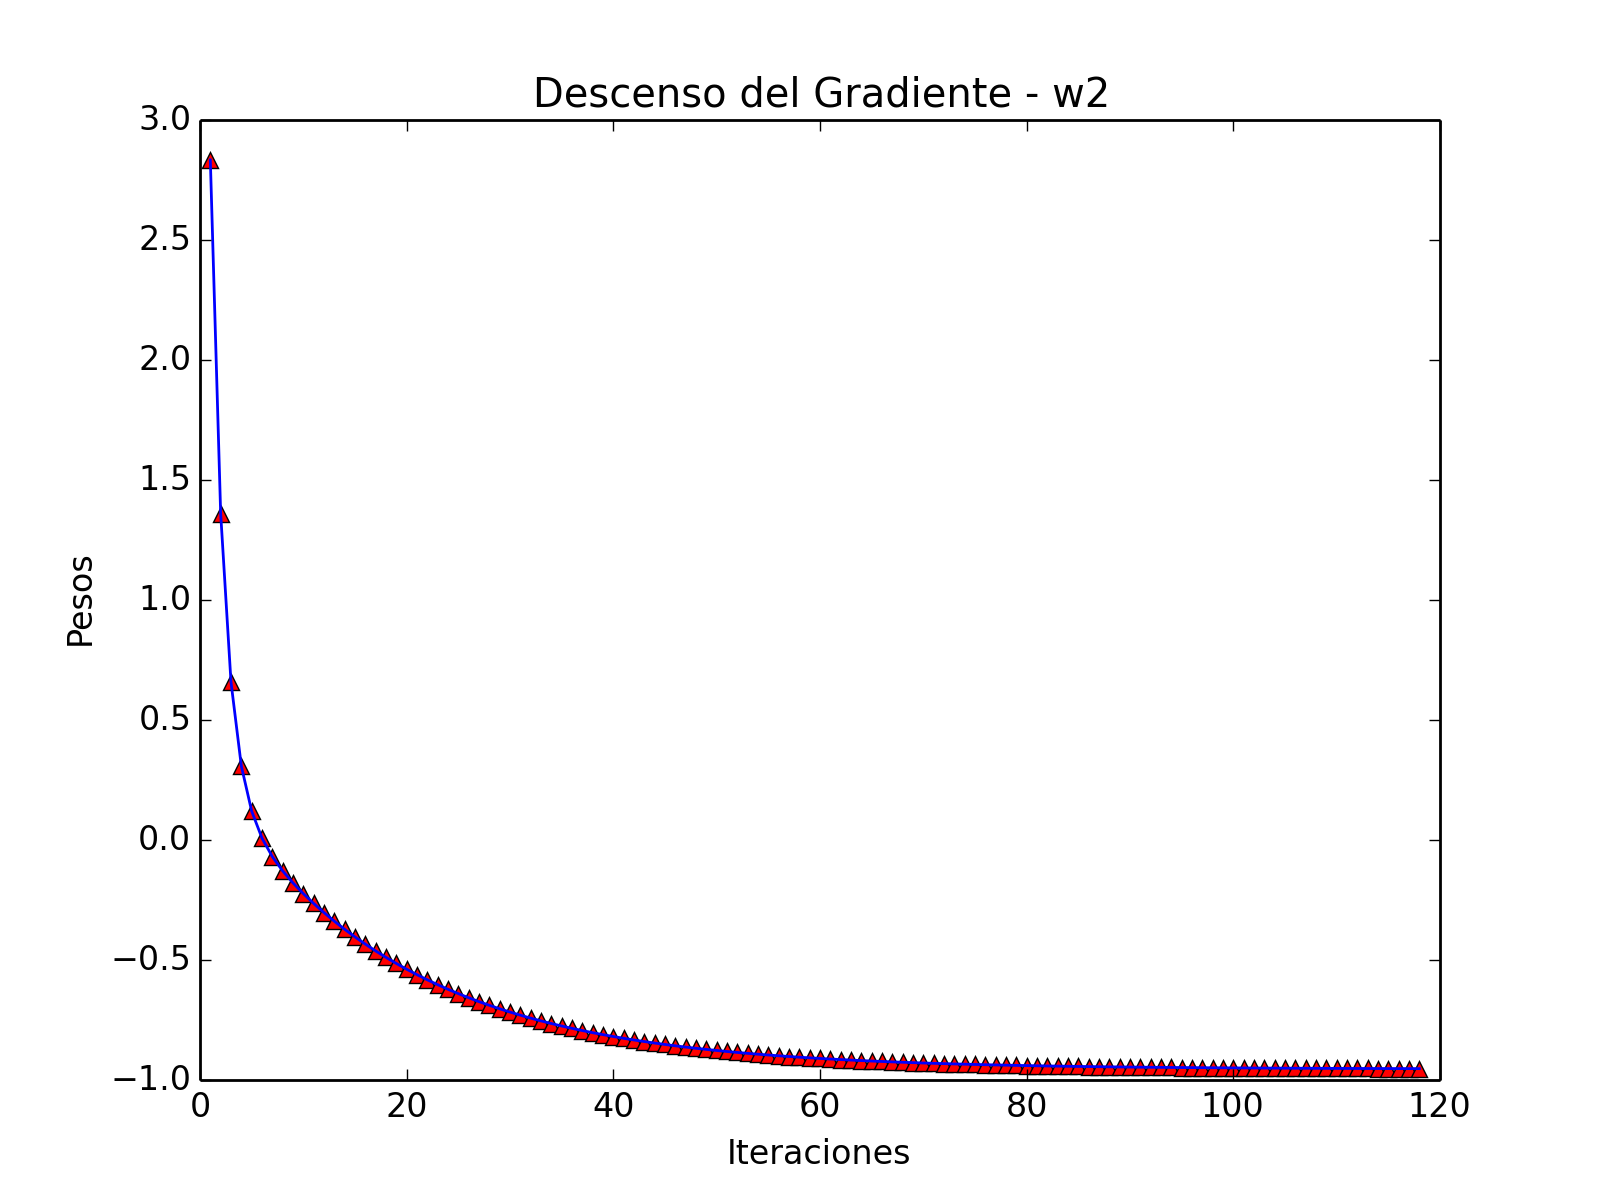
\includegraphics[scale=0.5]{gd2_2.png}
	\caption{Trayectoria de $w_{2}$}
	\label{f:gradient2_w2}
	\end{figure}
	
Al final el algoritmo con 0.0001 de precisión se obtuvo que el valor óptimo de w, donde E(w) es mínimo es $w = \left[\begin{array}{cc}
1.5973 & -0.9526
\end{array}\right]$, valores bastante cercanos a los que se calcularon directamente con el gradiente de la función.

\item $\eta = 1.0$\\
En las figura \ref{f:gradient1_w1} se encuentra la trayectoria de la evolución de $w_{1}$ durante las iteraciones realizadas por el algoritmo. Los puntos indican el valor específico que tuvo $w_{1}$ en cada iteración, y la línea es la trayectoria que realizó en total.

	\begin{figure}[H]
	\centering
	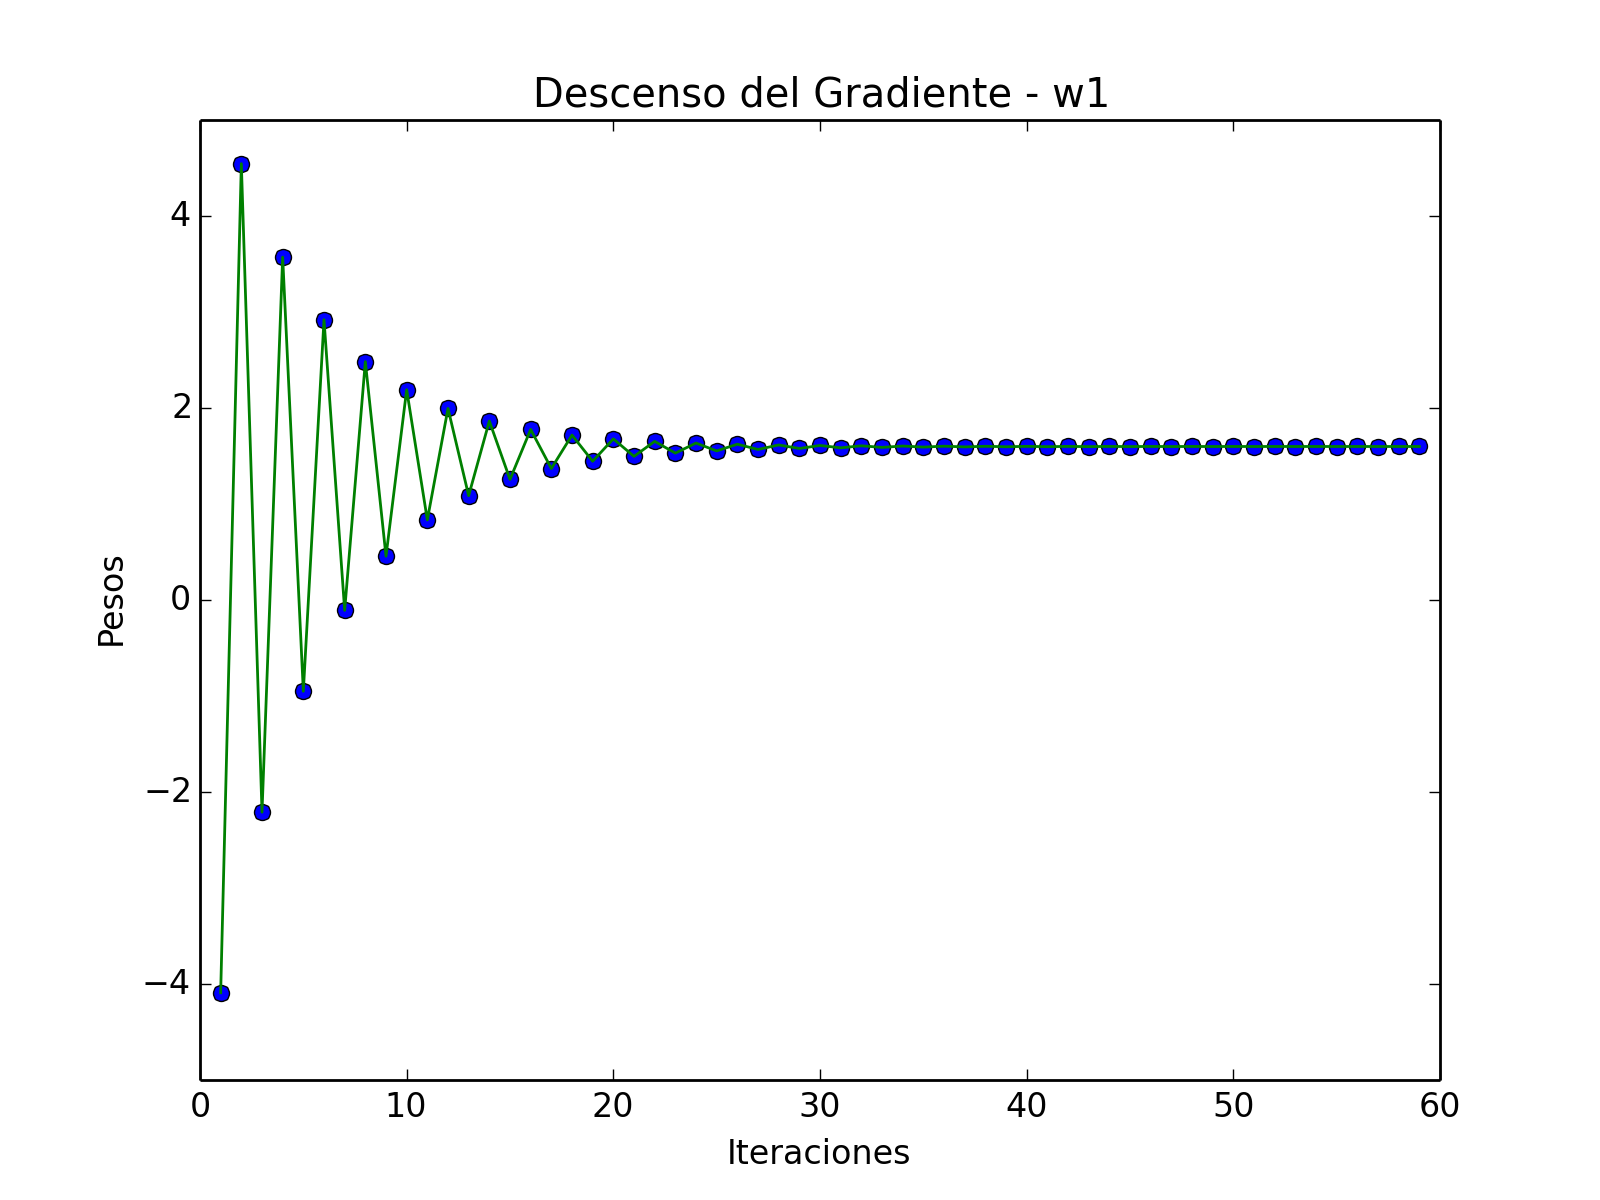
\includegraphics[scale=0.5]{gd1.png}
	\caption{Trayectoria de $w_{1}$}
	\label{f:gradient1_w1}
	\end{figure}

Además, en la figura \ref{f:gradient1_w2} se encuentran los valores por los que pasó $w_{2}$ durante las iteraciones, indicados por triángulos, junto a su trayectoria.

	\begin{figure}[H]
	\centering
	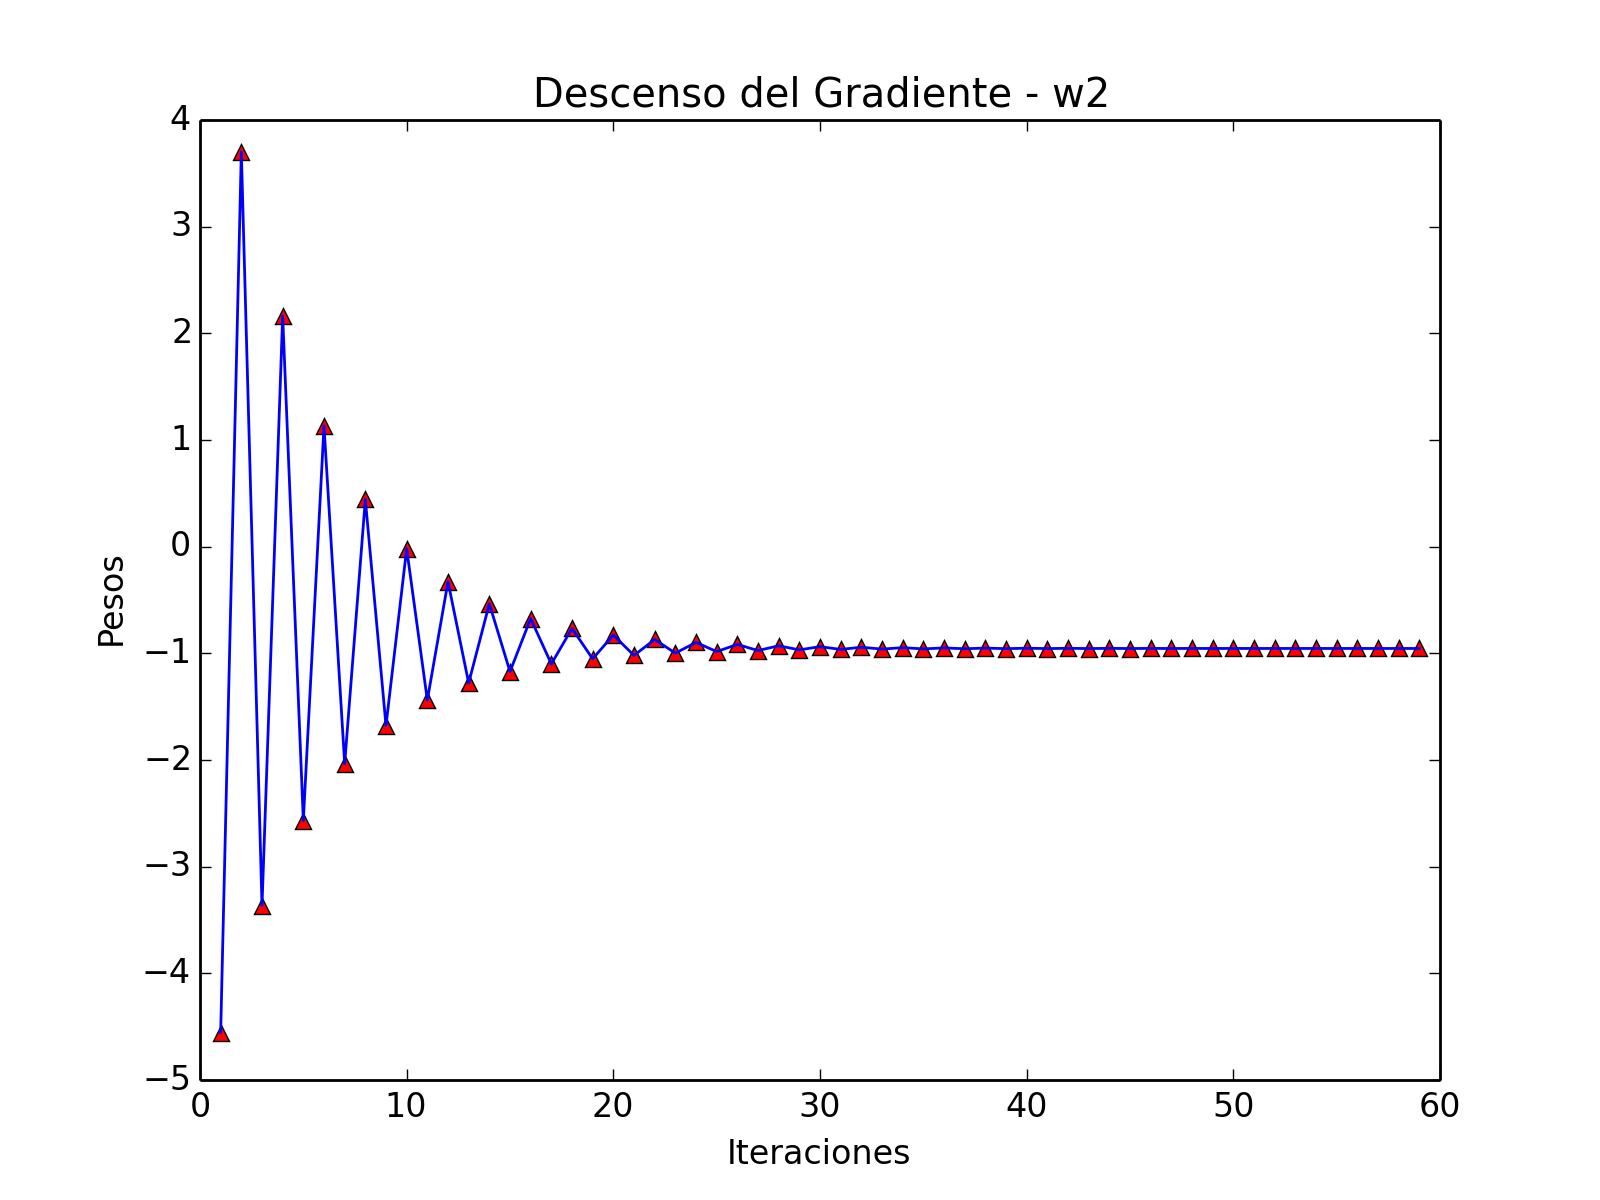
\includegraphics[scale=0.5]{gd2.png}
	\caption{Trayectoria de $w_{2}$}
	\label{f:gradient1_w2}
	\end{figure}
	
Al finalizar el algoritmo con 0.0001 de precisión se obtuvo que el valor óptimo w para el cual E(w) es mínimo es $w = \left[\begin{array}{cc}
1.5989 & -0.9543
\end{array}\right]$ siendo una aproximación casi exacta a la calculada en la primera parte.

\section{Detalles de implementación}
Todos los experimentos de esta tarea fueron implementados en \textit{Python 3}. Para el manejo de los arreglos de pesos y su generación aleatoria se usó la librería \textit{Numpy} y para las gráficas la librería \textit{Matplotlib}. La implementación de la validación cruzada fue realizada de forma manual, y los algoritmos del perceptrón y Adaline están basados en el código de los mismos implementado en \textit{Matlab} que se encuentra en el Aula Virtual.

\end{itemize}

\end{document}
